% subagent-routing-bench — A4 portrait one-pager, in the format of the scholastic-llm poster
% (published as docs/poster.pdf → pleyva2004.github.io/subagent-routing-bench/poster.pdf)

\documentclass[a4paper,9pt]{extarticle}

\usepackage[T1]{fontenc}
\usepackage{lmodern}
\usepackage[
  paper=a4paper,
  top=1.2cm, bottom=1.2cm,
  left=1.4cm, right=1.4cm,
  headsep=0.3cm
]{geometry}
\usepackage{microtype}
\usepackage{amsmath}
\usepackage{graphicx}
\usepackage{booktabs}
\usepackage{enumitem}
\setlist{nosep, leftmargin=1.2em, topsep=2pt, partopsep=0pt}
\usepackage{multicol}
\usepackage{tikz}
\usetikzlibrary{arrows.meta,positioning,shapes.geometric,calc}
\usepackage{pgfplots}
\pgfplotsset{compat=1.18}
\usepackage{xcolor}
\definecolor{accent}{HTML}{5e3023}
\definecolor{boxbg}{HTML}{f4f0eb}
\usepackage[hidelinks,colorlinks=true,urlcolor=accent,linkcolor=accent]{hyperref}
\usepackage{titlesec}
\titleformat{\section}{\large\bfseries\color{accent}}{}{0pt}{}[\vspace{-0.55em}\noindent\textcolor{accent!40}{\rule{\linewidth}{0.6pt}}]
\titlespacing*{\section}{0pt}{1.1em}{0.35em}
\titleformat{\subsection}{\normalsize\bfseries}{}{0pt}{}
\titlespacing*{\subsection}{0pt}{0.3em}{0.1em}
\pagestyle{empty}

% tighten line spacing
\linespread{1.02}
\setlength{\parskip}{2pt}
\setlength{\columnsep}{0.6cm}

\begin{document}

% ---------------------------------------------------------------------------
% Header
% ---------------------------------------------------------------------------
\begin{center}
  {\Large\bfseries\color{accent} Routing Claude Code Sub-Agents by Model and Effort}\\[2pt]
  {\small\itshape A Case Study of Claude Haiku 5.5 and Claude Sonnet 5.5 as cmux Sub-Agents}\\[3pt]
  {\small Pablo Leyva \,$\cdot$\, R1 New Jersey Institute of Technology \,$\cdot$\,
    \href{https://github.com/pleyva2004/subagent-routing-bench}{github.com/pleyva2004/subagent-routing-bench}
    \,$\cdot$\,
    \href{https://pleyva2004.github.io/subagent-routing-bench/paper.pdf}{paper}}
\end{center}
\vspace{-0.4em}
\noindent\textcolor{accent!40}{\rule{\linewidth}{0.6pt}}

% ---------------------------------------------------------------------------
% Headline TL;DR box
% ---------------------------------------------------------------------------
\vspace{0.7em}
\noindent\fcolorbox{accent!30}{boxbg}{\parbox{\dimexpr\linewidth-2\fboxsep-2\fboxrule}{%
% BEGIN TLDR
\textbf{TL;DR.} On a private Python repository, Haiku \texttt{low} passed
\textbf{30/30} code changes across two sets; over all hard-set tasks, reviews included,
it cost \textbf{\$0.041} per success (29/30) against \textbf{\$0.207} for Sonnet \texttt{low}
(26/30). On coding, effort above \texttt{medium} added cost with no gain we could detect:
Sonnet \texttt{xhigh} cost \textbf{2.2--2.6$\times$} Sonnet \texttt{low} per success, though nearly
every task passed, so this may be a ceiling effect. Reviews and long tool-free reasoning
did separate configs: Sonnet \texttt{xhigh} traced \textbf{1,300} statements; \texttt{low} to
\texttt{high} first failed at 600.
% END TLDR
}}
\vspace{0.7em}

% ---------------------------------------------------------------------------
% Two-column body
% ---------------------------------------------------------------------------
\begin{multicols}{2}
\raggedcolumns

% BEGIN LEFT
\section*{Motivation}
An orchestrating agent fans work out to sub-agents and must pick a model and
an effort level for each. Both choices drive cost, wall-clock time, and answer
quality, yet what extra effort buys, and what each choice costs per
\emph{successful} task, is rarely measured. We measure both for Claude Haiku~5.5
and Sonnet~5.5 run as Claude Code sub-agents.

\section*{Harness}
\begin{center}
\resizebox{0.7\linewidth}{!}{% Vertical pipeline figure for the poster: five stages, top to bottom.
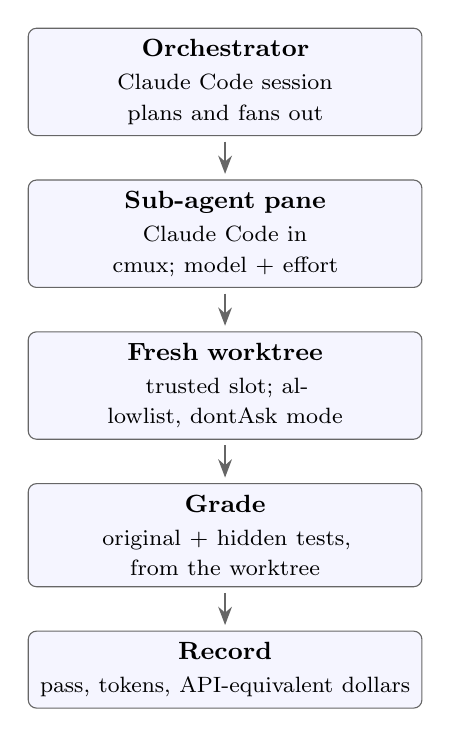
\begin{tikzpicture}[
    >=Stealth,
    box/.style={
      rectangle,
      rounded corners=3pt,
      draw=black!60,
      fill=blue!4,
      minimum height=0.9cm,
      minimum width=5.0cm,
      align=center,
      inner sep=4pt,
      text width=4.7cm,
      font=\small
    },
    arrow/.style={->, thick, draw=black!60, shorten <=2pt, shorten >=2pt, line width=0.8pt},
    node distance=0.55cm
  ]

  \node[box] (orch)   {\textbf{Orchestrator}\\[1pt]\footnotesize Claude Code session plans and fans out};
  \node[box, below=of orch]  (pane)   {\textbf{Sub-agent pane}\\[1pt]\footnotesize Claude Code in cmux; model + effort};
  \node[box, below=of pane]  (wt)     {\textbf{Fresh worktree}\\[1pt]\footnotesize trusted slot; allowlist, dontAsk mode};
  \node[box, below=of wt]    (grade)  {\textbf{Grade}\\[1pt]\footnotesize original + hidden tests, from the worktree};
  \node[box, below=of grade] (record) {\textbf{Record}\\[1pt]\footnotesize pass, tokens, API-equivalent dollars};

  \draw[arrow] (orch)  -- (pane);
  \draw[arrow] (pane)  -- (wt);
  \draw[arrow] (wt)    -- (grade);
  \draw[arrow] (grade) -- (record);

\end{tikzpicture}
}
\end{center}
\vspace{-0.4em}
\noindent Each sub-agent is a Claude Code session in a cmux pane, working in
a fresh git worktree under an allowlist. We grade from the worktree with hidden
tests and compute API-equivalent cost from the transcript.

\section*{Experiments}
\begin{itemize}
  \item \textbf{Reasoning ladder:} 3 families, 10 levels, 8 configs, 229 runs, no tools
  \item \textbf{Easy coding set:} 12 tasks (locate, fix, feature replay, review), all 10 configs, 120 runs
  \item \textbf{Hard coding set:} 10 tasks, 5 configs, 3 trials, 150 runs
  \item \textbf{Validation:} admission checks, model-verified briefs, an oracle self-test
  \item \textbf{Grading:} hidden tests, exact locations, planted-bug keys
  \item \textbf{Cost:} coding runs about \$24 (easy) and \$34 (hard)
\end{itemize}
% END LEFT

\columnbreak

% BEGIN RIGHT
\section*{Results}
\begin{center}
\resizebox{0.95\linewidth}{!}{% Grouped bars: dollars per success by config, easy vs hard set.
% Generated by analysis/make_poster_figures.py from data/coding/costs.json.
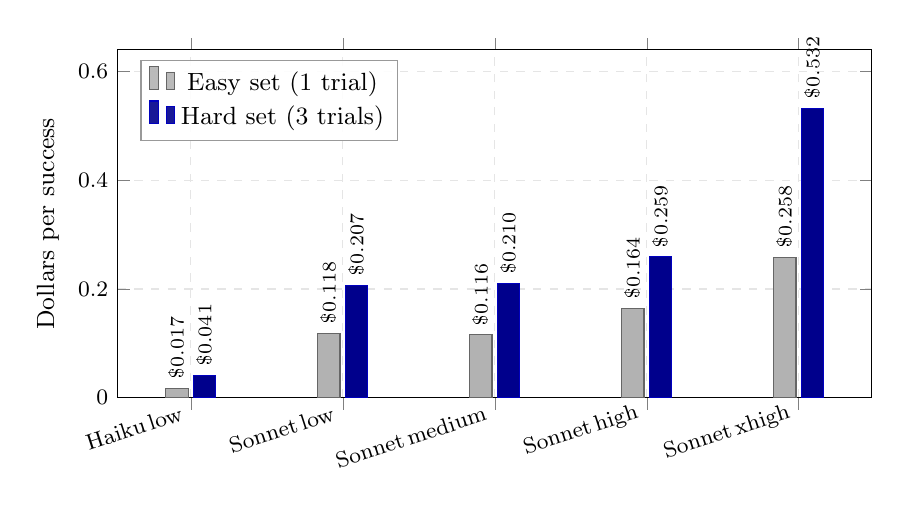
\begin{tikzpicture}
\begin{axis}[
    width=0.92\linewidth,
    height=6cm,
    ybar,
    bar width=8pt,
    ymin=0, ymax=0.64,
    enlarge x limits=0.12,
    ylabel={Dollars per success},
    symbolic x coords={Haiku\,low, Sonnet\,low, Sonnet\,medium, Sonnet\,high, Sonnet\,xhigh},
    xtick=data,
    x tick label style={font=\footnotesize, rotate=18, anchor=east},
    tick label style={font=\footnotesize},
    label style={font=\small},
    nodes near coords={\$\pgfmathprintnumber[fixed,fixed zerofill,precision=3]{\pgfplotspointmeta}},
    point meta=rawy,
    nodes near coords style={font=\scriptsize, rotate=90, anchor=west},
    legend pos=north west,
    legend style={font=\small,fill=white,fill opacity=0.9,text opacity=1,draw=black!40},
    grid=major,
    grid style={dashed,gray!20},
  ]

  \addplot[fill=gray!60, draw=gray!80!black] coordinates {
    (Haiku\,low, 0.0174)
    (Sonnet\,low, 0.1184)
    (Sonnet\,medium, 0.1156)
    (Sonnet\,high, 0.1638)
    (Sonnet\,xhigh, 0.2584)
  };
  \addlegendentry{Easy set (1 trial)}

  \addplot[fill=blue!55!black, draw=blue!75!black] coordinates {
    (Haiku\,low, 0.041)
    (Sonnet\,low, 0.2071)
    (Sonnet\,medium, 0.2097)
    (Sonnet\,high, 0.2593)
    (Sonnet\,xhigh, 0.5323)
  };
  \addlegendentry{Hard set (3 trials)}

\end{axis}
\end{tikzpicture}
}
\end{center}
\vspace{-0.6em}

\noindent Dollars per success for the five configs run in both sets. Hard-set pass
rates as graded: Haiku \texttt{low} \textbf{29/30}, Sonnet \textbf{26--27/30} (intervals overlap).
Code changes: Haiku \texttt{low} \textbf{30/30} across both sets. Code-trace
thresholds (statements): Haiku \texttt{low} \textbf{80}, Sonnet
\texttt{low}/\texttt{medium} \textbf{400}, Sonnet \texttt{xhigh} \textbf{1,300+}.

\section*{Where configs failed}
\begin{itemize}
  \item \textbf{Swap shortcut.} At 40 statements, Haiku \texttt{high} and
    \texttt{xhigh} read three swaps of one pair plus one of another as
    ``four swaps that cancel''; \texttt{low} and \texttt{medium} traced each line.
  \item \textbf{Shutdown-loop review bug.} Every Haiku level and Sonnet
    \texttt{xhigh} missed it, citing a real nearby flaw instead.
  \item \textbf{Broadened error handler.} No Sonnet run flagged it (arguably a
    robustness choice); Haiku \texttt{low} did in 2 of 3, too few to call it better.
\end{itemize}
\noindent Hypothesis: a second model catches what more effort does not. It
rests on a handful of cases, with exceptions in both directions.

\section*{Routing \& takeaway}
\begin{itemize}
  \item Lookups and code changes: Haiku \texttt{low}
  \item Sonnet \texttt{medium} when wall-clock time matters
  \item Review: both models in parallel, merge findings (a hypothesis)
  \item Long tool-free reasoning: Sonnet \texttt{xhigh}
  \item \texttt{max} only on explicit request
\end{itemize}

\smallskip\noindent\textbf{Takeaway.} Choose the cheapest model that clears the
task; on coding, more effort rarely paid, and a second model may be more useful than a
higher level. Main caveat: one private repository, and nearly every task
passed everywhere, so we did not find where coding reliability breaks down.
% END RIGHT

\end{multicols}

% ---------------------------------------------------------------------------
% Compact single-band footer pushed to the bottom by \vfill
% ---------------------------------------------------------------------------
\vfill
\noindent\textcolor{accent!40}{\rule{\linewidth}{0.6pt}}

\vspace{0.15em}
\noindent\footnotesize%
\href{https://github.com/pleyva2004/subagent-routing-bench}{\textbf{Repo}}\,\textbar{}\,%
\href{https://pleyva2004.github.io/subagent-routing-bench/paper.pdf}{\textbf{Paper}}\,\textbar{}\,%
\href{mailto:pleyva2004@gmail.com}{\textbf{Contact}}\quad
\emph{Case study on one private repository; dollar figures are API-equivalent estimates.}
\normalsize

\end{document}
